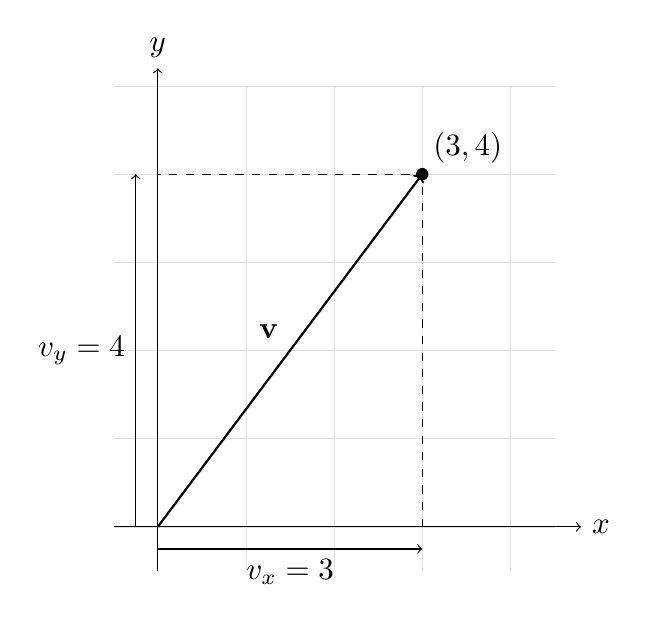
\begin{tikzpicture}[scale=1.12, transform shape]
    \draw[step=1, gray!25, very thin] (-0.5,-0.5) grid (4.5,5.0);
    \draw[->] (-0.5,0) -- (4.8,0) node[right] {$x$};
    \draw[->] (0,-0.5) -- (0,5.2) node[above] {$y$};
    \draw[->, thick] (0,0) -- (3,4) node[midway, above left] {$\mathbf{v}$};
    \draw[dashed] (3,0) -- (3,4) -- (0,4);
    \draw[->] (0,-0.25) -- (3,-0.25) node[midway, below] {$v_x=3$};
    \draw[->] (-0.25,0) -- (-0.25,4) node[midway, left] {$v_y=4$};
    \fill (3,4) circle (2pt);
    \node[above right] at (3,4) {$(3,4)$};
\end{tikzpicture}
